\documentclass[]{article}
\usepackage{lmodern}
\usepackage{amssymb,amsmath}
\usepackage{ifxetex,ifluatex}
\usepackage{fixltx2e} % provides \textsubscript
\ifnum 0\ifxetex 1\fi\ifluatex 1\fi=0 % if pdftex
  \usepackage[T1]{fontenc}
  \usepackage[utf8]{inputenc}
\else % if luatex or xelatex
  \ifxetex
    \usepackage{mathspec}
  \else
    \usepackage{fontspec}
  \fi
  \defaultfontfeatures{Ligatures=TeX,Scale=MatchLowercase}
\fi
% use upquote if available, for straight quotes in verbatim environments
\IfFileExists{upquote.sty}{\usepackage{upquote}}{}
% use microtype if available
\IfFileExists{microtype.sty}{%
\usepackage{microtype}
\UseMicrotypeSet[protrusion]{basicmath} % disable protrusion for tt fonts
}{}
\usepackage[margin=1in]{geometry}
\usepackage{hyperref}
\hypersetup{unicode=true,
            pdftitle={Laborator 4},
            pdfborder={0 0 0},
            breaklinks=true}
\urlstyle{same}  % don't use monospace font for urls
\usepackage{color}
\usepackage{fancyvrb}
\newcommand{\VerbBar}{|}
\newcommand{\VERB}{\Verb[commandchars=\\\{\}]}
\DefineVerbatimEnvironment{Highlighting}{Verbatim}{commandchars=\\\{\}}
% Add ',fontsize=\small' for more characters per line
\usepackage{framed}
\definecolor{shadecolor}{RGB}{248,248,248}
\newenvironment{Shaded}{\begin{snugshade}}{\end{snugshade}}
\newcommand{\KeywordTok}[1]{\textcolor[rgb]{0.13,0.29,0.53}{\textbf{#1}}}
\newcommand{\DataTypeTok}[1]{\textcolor[rgb]{0.13,0.29,0.53}{#1}}
\newcommand{\DecValTok}[1]{\textcolor[rgb]{0.00,0.00,0.81}{#1}}
\newcommand{\BaseNTok}[1]{\textcolor[rgb]{0.00,0.00,0.81}{#1}}
\newcommand{\FloatTok}[1]{\textcolor[rgb]{0.00,0.00,0.81}{#1}}
\newcommand{\ConstantTok}[1]{\textcolor[rgb]{0.00,0.00,0.00}{#1}}
\newcommand{\CharTok}[1]{\textcolor[rgb]{0.31,0.60,0.02}{#1}}
\newcommand{\SpecialCharTok}[1]{\textcolor[rgb]{0.00,0.00,0.00}{#1}}
\newcommand{\StringTok}[1]{\textcolor[rgb]{0.31,0.60,0.02}{#1}}
\newcommand{\VerbatimStringTok}[1]{\textcolor[rgb]{0.31,0.60,0.02}{#1}}
\newcommand{\SpecialStringTok}[1]{\textcolor[rgb]{0.31,0.60,0.02}{#1}}
\newcommand{\ImportTok}[1]{#1}
\newcommand{\CommentTok}[1]{\textcolor[rgb]{0.56,0.35,0.01}{\textit{#1}}}
\newcommand{\DocumentationTok}[1]{\textcolor[rgb]{0.56,0.35,0.01}{\textbf{\textit{#1}}}}
\newcommand{\AnnotationTok}[1]{\textcolor[rgb]{0.56,0.35,0.01}{\textbf{\textit{#1}}}}
\newcommand{\CommentVarTok}[1]{\textcolor[rgb]{0.56,0.35,0.01}{\textbf{\textit{#1}}}}
\newcommand{\OtherTok}[1]{\textcolor[rgb]{0.56,0.35,0.01}{#1}}
\newcommand{\FunctionTok}[1]{\textcolor[rgb]{0.00,0.00,0.00}{#1}}
\newcommand{\VariableTok}[1]{\textcolor[rgb]{0.00,0.00,0.00}{#1}}
\newcommand{\ControlFlowTok}[1]{\textcolor[rgb]{0.13,0.29,0.53}{\textbf{#1}}}
\newcommand{\OperatorTok}[1]{\textcolor[rgb]{0.81,0.36,0.00}{\textbf{#1}}}
\newcommand{\BuiltInTok}[1]{#1}
\newcommand{\ExtensionTok}[1]{#1}
\newcommand{\PreprocessorTok}[1]{\textcolor[rgb]{0.56,0.35,0.01}{\textit{#1}}}
\newcommand{\AttributeTok}[1]{\textcolor[rgb]{0.77,0.63,0.00}{#1}}
\newcommand{\RegionMarkerTok}[1]{#1}
\newcommand{\InformationTok}[1]{\textcolor[rgb]{0.56,0.35,0.01}{\textbf{\textit{#1}}}}
\newcommand{\WarningTok}[1]{\textcolor[rgb]{0.56,0.35,0.01}{\textbf{\textit{#1}}}}
\newcommand{\AlertTok}[1]{\textcolor[rgb]{0.94,0.16,0.16}{#1}}
\newcommand{\ErrorTok}[1]{\textcolor[rgb]{0.64,0.00,0.00}{\textbf{#1}}}
\newcommand{\NormalTok}[1]{#1}
\usepackage{longtable,booktabs}
\usepackage{graphicx,grffile}
\makeatletter
\def\maxwidth{\ifdim\Gin@nat@width>\linewidth\linewidth\else\Gin@nat@width\fi}
\def\maxheight{\ifdim\Gin@nat@height>\textheight\textheight\else\Gin@nat@height\fi}
\makeatother
% Scale images if necessary, so that they will not overflow the page
% margins by default, and it is still possible to overwrite the defaults
% using explicit options in \includegraphics[width, height, ...]{}
\setkeys{Gin}{width=\maxwidth,height=\maxheight,keepaspectratio}
\IfFileExists{parskip.sty}{%
\usepackage{parskip}
}{% else
\setlength{\parindent}{0pt}
\setlength{\parskip}{6pt plus 2pt minus 1pt}
}
\setlength{\emergencystretch}{3em}  % prevent overfull lines
\providecommand{\tightlist}{%
  \setlength{\itemsep}{0pt}\setlength{\parskip}{0pt}}
\setcounter{secnumdepth}{5}
% Redefines (sub)paragraphs to behave more like sections
\ifx\paragraph\undefined\else
\let\oldparagraph\paragraph
\renewcommand{\paragraph}[1]{\oldparagraph{#1}\mbox{}}
\fi
\ifx\subparagraph\undefined\else
\let\oldsubparagraph\subparagraph
\renewcommand{\subparagraph}[1]{\oldsubparagraph{#1}\mbox{}}
\fi

%%% Use protect on footnotes to avoid problems with footnotes in titles
\let\rmarkdownfootnote\footnote%
\def\footnote{\protect\rmarkdownfootnote}

%%% Change title format to be more compact
\usepackage{titling}

% Create subtitle command for use in maketitle
\newcommand{\subtitle}[1]{
  \posttitle{
    \begin{center}\large#1\end{center}
    }
}

\setlength{\droptitle}{-2em}
  \title{Laborator 4}
  \pretitle{\vspace{\droptitle}\centering\huge}
  \posttitle{\par}
\subtitle{Exerciții de probabilități în R}
  \author{}
  \preauthor{}\postauthor{}
  \date{}
  \predate{}\postdate{}

\usepackage{booktabs}
\usepackage{longtable}
\usepackage{framed,color}
\definecolor{shadecolor}{RGB}{248, 248, 248}
\definecolor{shadecolor1}{RGB}{216,225,235}
\definecolor{framecolor}{RGB}{108,123,13}

\ifxetex
  \usepackage{letltxmacro}
  \setlength{\XeTeXLinkMargin}{1pt}
  \LetLtxMacro\SavedIncludeGraphics\includegraphics
  \def\includegraphics#1#{% #1 catches optional stuff (star/opt. arg.)
    \IncludeGraphicsAux{#1}%
  }%
  \newcommand*{\IncludeGraphicsAux}[2]{%
    \XeTeXLinkBox{%
      \SavedIncludeGraphics#1{#2}%
    }%
  }%
\fi

\newenvironment{frshaded*}{%
  \def\FrameCommand{\fboxrule=\FrameRule\fboxsep=\FrameSep \fcolorbox{framecolor}{shadecolor1}}%
  \MakeFramed {\advance\hsize-\width \FrameRestore}}%
{\endMakeFramed}

\newenvironment{rmdblock}[1]
  {\begin{frshaded*}
  \begin{itemize}
  \renewcommand{\labelitemi}{
    \raisebox{-.7\height}[0pt][0pt]{
      {\setkeys{Gin}{width=2em,keepaspectratio}\includegraphics{images/icons/#1}}
    }
  }
  \item
  }
  {
  \end{itemize}
  \end{frshaded*}
  }
  
\newenvironment{rmdcaution}
  {\begin{rmdblock}{caution}}
  {\end{rmdblock}}
% \newenvironment{rmdinsight}
%   {\begin{rmdblock}{insight}}
%   {\end{rmdblock}}
\newenvironment{rmdexercise}
  {\begin{rmdblock}{exercise}}
  {\end{rmdblock}}
\newenvironment{rmdtip}
  {\begin{rmdblock}{tip}}
  {\end{rmdblock}}
  
  
%%%%%%%%%%%%%%%%%%%%%%%%%%%%%%%%%%%%%%%%%%%%%%%%%%%%%%%%%%%%%%%%%%%%%%%%%%%%%%%%%%%%%%%%%%%%%%%%%%%%%%%%%%%%%%%%%%%%%
%%%%%%%%%%% For insight block %%%%%%%%%%%%%%%%%%%%%%%%%%
\definecolor{shadecolor_insight}{RGB}{223,240,216}
\definecolor{framecolor_insight}{RGB}{136,193,137}

\newenvironment{frshaded_insight*}{%
  \def\FrameCommand{\fboxrule=\FrameRule\fboxsep=\FrameSep \fcolorbox{framecolor_insight}{shadecolor_insight}}%
  \MakeFramed {\advance\hsize-\width \FrameRestore}}%
{\endMakeFramed}

\newenvironment{rmdblock_insight}[1]
  {\begin{frshaded_insight*}
  \begin{itemize}
  \renewcommand{\labelitemi}{
    \raisebox{-.7\height}[0pt][0pt]{
      {\setkeys{Gin}{width=2em,keepaspectratio}\includegraphics{images/icons/#1}}
    }
  }
  \item
  }
  {
  \end{itemize}
  \end{frshaded_insight*}
  }
  
\newenvironment{rmdinsight}
  {\begin{rmdblock_insight}{insight}}
  {\end{rmdblock_insight}}
  
%%%%%%%%%%%%%%%%%%%%%%%%%%%%%%%%%%%%%%%%%%%%%%%%%%%%%%%%%%%%%%%%%%%%%%%%%%%%%%%%%%%%%%%%%%%%%%%%%%%%%%%%%%%%%%%%%%%%%
\usepackage{subfigure}
\usepackage{booktabs}
\usepackage{slashbox}
\usepackage{color}
%%%%%%%%%%%%%%%%%%%%%%%%%%%%%%%%%%%%%%%%%%%%%%%%%%%%%%%%%%%%%%%%%%%%%%%%%%%%%%%%%%%%%%%%%%%%%%%%%%%%%%%%%%%%%%%%%%%%%
%CITEVA DEFINITII
\def\om{\omega}
\def\Om{\Omega}
\def\et{\eta}
\def\td{\tilde{\delta}}
\def\m{{\mu}}
\def\n{{\nu}}
\def\k{{\kappa}}
\def\l{{\lambda}}
\def\L{{\Lambda}}
\def\g{{\gamma}}
\def\a{{\alpha}}
\def\e{{\varepsilon}}
\def\b{{\beta}}
\def\G{{\Gamma}}
\def\d{{\delta}}
\def\D{{\Delta}}
\def\t{{\theta}}
\def\s{{\sigma}}
\def\S{{\Sigma}}
\def\z{{\zeta}}
\def\qed{\hfill\Box}
\def\ds{\displaystyle}
\def\mc{\mathcal}
%%%%%%%%%%%%%%%%%%%%%%%%%%%%%%%%%%%%%%%%%%%%%%%%%%%%%%%%%%%%%%%%%%%%%%%%%%%%%%%%%%%%%%%%%%%%%%%%%%%%%%%%%%%%%%%%%%%%%%
\def\1{{\mathbf 1}}
\def\CC{{\mathbb C}}
\def\VV{{\mathbb V}}
\def\RR{{\mathbb R}}
\def\QQ{{\mathbb Q}}
\def\ZZ{{\mathbb Z}}
\def\PP{{\mathbb P}}
\def\EE{{\mathbb E}}
\def\NN{{\mathbb N}}
\def\FF{{\mathbb F}}
%\def\SS{{\mathbb S}}
\def\MA{{\mathcal A}}
\def\MO{{\mathcal O}}
\def\MF{{\mathcal F}}
\def\ME{{\mathcal E}}
\def\MR{{\mathcal R}}
\def\MB{{\mathcal B}}
\def\MM{{\mathcal M}}
\def\MN{{\mathcal N}}
\def\MU{{\mathcal U}}
\def\MP{{\mathcal P}}
\def\MS{{\mathcal S}}
\def\MBS{{\mathbf S}}
\def\MX{{\bm{ \mathscr X}}}

% independent sign
\newcommand\independent{\protect\mathpalette{\protect\independenT}{\perp}}
\def\independenT#1#2{\mathrel{\rlap{$#1#2$}\mkern2mu{#1#2}}}

\renewcommand\tablename{Tab.}
\renewcommand{\figurename}{Fig.}

%%%%%%%%%%%%%%%%%%%%%%%%%%%%%%%%%%%%%%%%%%%%%%%%%%%%%%%%%%%%%%%%%%%%%%%%%%%%%%%%%%%%%%%%%%%%%%%%%%%%%%%%%%%%%%%%%%%%%
%Header and Footer
\usepackage{fancyhdr}

\pagestyle{fancy}
\fancyhf{}
\rhead{Universitatea din Bucure\c sti\\ Facultatea de Matematic\u a \c si Informatic\u a}
\lhead{\textit{Curs}: Probabilit\u a\c ti \c si Statistic\u a\\ \textit{Instructor}: A. Am\u arioarei}
\rfoot{Pagina \thepage}
\lfoot{Grupele: 241, 242, 243, 244}
%%%%%%%%%%%%%%%%%%%%%%%%%%%%%%%%%%%%%%%

\begin{document}
\maketitle

%%%%%%%%%%%%%%%%%%%%%%%%
\thispagestyle{fancy}

Obiectivul acestui laborator este de a rezolva câteva probleme de teoria
probabilităților cu ajutorul limbajului R.

\section{Generarea unei variabile aleatoare
discrete}\label{generarea-unei-variabile-aleatoare-discrete}

\begin{rmdexercise}
Definiți o funcție care să genereze un eșantion de talie \(n\) dintr-o
distribuție discretă definită pe mulțimea \(\{x_1,\dots,x_N\}\) cu
probabilitățile \(\{p_1,\dots,p_N\}\). Pentru început încercați cu v.a.
de tip Bernoulli.
\end{rmdexercise}

Avem următoarea funcție:

\begin{Shaded}
\begin{Highlighting}[]
\NormalTok{GenerateDiscrete =}\StringTok{ }\ControlFlowTok{function}\NormalTok{(}\DataTypeTok{n =} \DecValTok{1}\NormalTok{, x, p, }\DataTypeTok{err =} \FloatTok{1e-15}\NormalTok{)\{}
  \CommentTok{# talia esantionului}
  \CommentTok{# x alfabetul }
  \CommentTok{# p probabilitatile}
\NormalTok{  lp =}\StringTok{ }\KeywordTok{length}\NormalTok{(p)}
\NormalTok{  lx =}\StringTok{ }\KeywordTok{length}\NormalTok{(x)}
  
  \CommentTok{# verify if x and p have the same size }
  \ControlFlowTok{if}\NormalTok{(}\KeywordTok{abs}\NormalTok{(}\KeywordTok{sum}\NormalTok{(p)}\OperatorTok{-}\DecValTok{1}\NormalTok{)}\OperatorTok{>}\NormalTok{err }\OperatorTok{|}\StringTok{ }\KeywordTok{sum}\NormalTok{(p}\OperatorTok{>=}\DecValTok{0}\NormalTok{)}\OperatorTok{!=}\NormalTok{lp)\{}
    
    \KeywordTok{stop}\NormalTok{(}\StringTok{"suma probabilitatilor nu este 1 sau probabilitatile sunt mai mici decat 0"}\NormalTok{)}
    
\NormalTok{  \}}\ControlFlowTok{else} \ControlFlowTok{if}\NormalTok{(lx}\OperatorTok{!=}\NormalTok{lp)\{}
    
    \KeywordTok{stop}\NormalTok{(}\StringTok{"x si p ar trebui sa aiba aceeasi marime"}\NormalTok{)}
    
\NormalTok{  \}}\ControlFlowTok{else}\NormalTok{\{}
\NormalTok{    out =}\StringTok{ }\KeywordTok{rep}\NormalTok{(}\DecValTok{0}\NormalTok{, n)}
    
\NormalTok{    indOrderProb =}\StringTok{ }\KeywordTok{order}\NormalTok{(p, }\DataTypeTok{decreasing =} \OtherTok{TRUE}\NormalTok{) }\CommentTok{# index}
\NormalTok{    pOrdered =}\StringTok{ }\NormalTok{p[indOrderProb] }\CommentTok{# rearrange the values of the probabilities }
\NormalTok{    xOrdered =}\StringTok{ }\NormalTok{x[indOrderProb] }\CommentTok{# rearramnge the values of x}
    
    \CommentTok{# u = runif(n) # generate n uniforms}
\NormalTok{    pOrderedCS =}\StringTok{ }\KeywordTok{cumsum}\NormalTok{(pOrdered)}
    
    \ControlFlowTok{for}\NormalTok{ (i }\ControlFlowTok{in} \DecValTok{1}\OperatorTok{:}\NormalTok{n)\{}
\NormalTok{      u =}\StringTok{ }\KeywordTok{runif}\NormalTok{(}\DecValTok{1}\NormalTok{)}
      
\NormalTok{      k =}\StringTok{ }\KeywordTok{min}\NormalTok{(}\KeywordTok{which}\NormalTok{(u}\OperatorTok{<=}\NormalTok{pOrderedCS))}
\NormalTok{      out[i] =}\StringTok{ }\NormalTok{xOrdered[k]}
\NormalTok{    \}}
\NormalTok{  \}}
  
  \KeywordTok{return}\NormalTok{(out)}
\NormalTok{\}}
\end{Highlighting}
\end{Shaded}

și pentru a o putea testa să considerăm cazul repartițiilor Poisson și
Geometrică:

\begin{enumerate}
\def\labelenumi{\alph{enumi})}
\tightlist
\item
  Poisson
\end{enumerate}

\begin{Shaded}
\begin{Highlighting}[]
\CommentTok{# Poisson}
\KeywordTok{hist}\NormalTok{(}\KeywordTok{GenerateDiscrete}\NormalTok{(}\DecValTok{10000}\NormalTok{, }\DataTypeTok{x =} \DecValTok{0}\OperatorTok{:}\DecValTok{50}\NormalTok{, }
                      \DataTypeTok{p =} \KeywordTok{dpois}\NormalTok{(}\DecValTok{0}\OperatorTok{:}\DecValTok{50}\NormalTok{, }\DecValTok{5}\NormalTok{)), }
     \DataTypeTok{probability =} \OtherTok{TRUE}\NormalTok{, }
     \DataTypeTok{breaks =} \KeywordTok{seq}\NormalTok{(}\OperatorTok{-}\FloatTok{0.5}\NormalTok{,}\FloatTok{49.5}\NormalTok{, }\DataTypeTok{by =} \DecValTok{1}\NormalTok{), }
     \DataTypeTok{xlim =} \KeywordTok{c}\NormalTok{(}\OperatorTok{-}\FloatTok{0.5}\NormalTok{, }\DecValTok{20}\NormalTok{),}
     \DataTypeTok{col =} \StringTok{"grey80"}\NormalTok{,}
     \DataTypeTok{main =} \StringTok{"Repartitia Poisson"}\NormalTok{,}
     \DataTypeTok{xlab =} \StringTok{"X"}\NormalTok{,}
     \DataTypeTok{ylab =} \StringTok{"Densitatea"}\NormalTok{)}

\KeywordTok{lines}\NormalTok{(}\DecValTok{0}\OperatorTok{:}\DecValTok{50}\NormalTok{,}
      \KeywordTok{dpois}\NormalTok{(}\DecValTok{0}\OperatorTok{:}\DecValTok{50}\NormalTok{, }\DecValTok{5}\NormalTok{), }
      \DataTypeTok{type =} \StringTok{"l"}\NormalTok{, }
      \DataTypeTok{col =} \StringTok{"brown3"}\NormalTok{, }\DataTypeTok{lty =} \DecValTok{2}\NormalTok{, }\DataTypeTok{lwd =} \DecValTok{2}\NormalTok{)}
\end{Highlighting}
\end{Shaded}

\begin{center}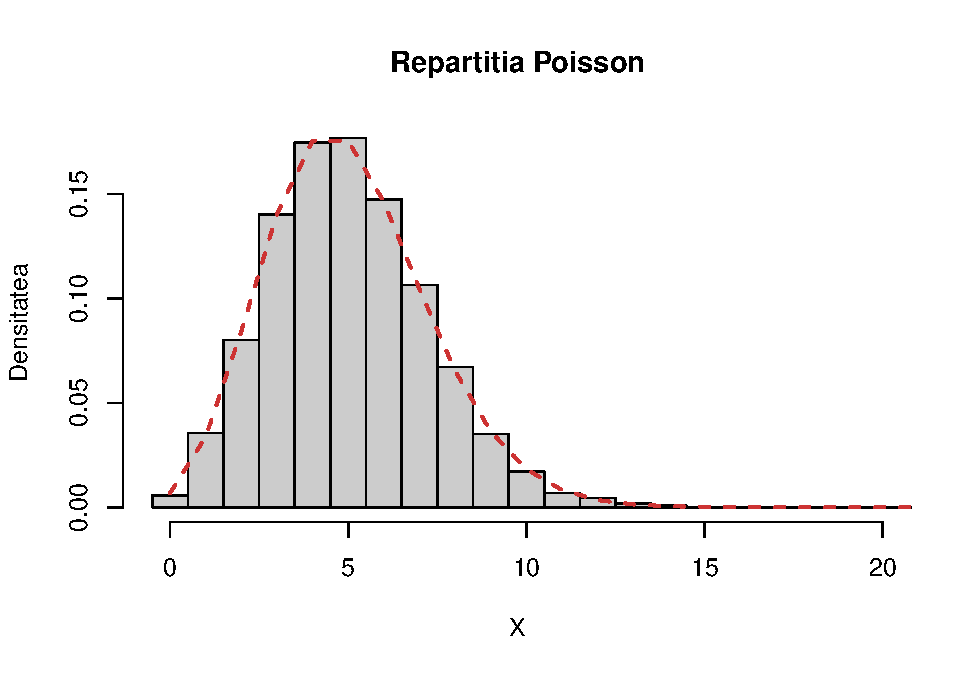
\includegraphics{Lab_4_files/figure-latex/unnamed-chunk-4-1} \end{center}

\begin{enumerate}
\def\labelenumi{\alph{enumi})}
\setcounter{enumi}{1}
\tightlist
\item
  Geometrică
\end{enumerate}

\begin{Shaded}
\begin{Highlighting}[]
\CommentTok{# Geometric}
\KeywordTok{hist}\NormalTok{(}\KeywordTok{GenerateDiscrete}\NormalTok{(}\DecValTok{10000}\NormalTok{, }\DataTypeTok{x =} \DecValTok{0}\OperatorTok{:}\DecValTok{100}\NormalTok{, }
                      \DataTypeTok{p =} \KeywordTok{dgeom}\NormalTok{(}\DecValTok{0}\OperatorTok{:}\DecValTok{100}\NormalTok{, }\FloatTok{0.3}\NormalTok{)), }
     \DataTypeTok{probability =} \OtherTok{TRUE}\NormalTok{, }
     \DataTypeTok{breaks =} \KeywordTok{seq}\NormalTok{(}\OperatorTok{-}\FloatTok{0.5}\NormalTok{,}\FloatTok{99.5}\NormalTok{, }\DataTypeTok{by =} \DecValTok{1}\NormalTok{),}
     \DataTypeTok{xlim =} \KeywordTok{c}\NormalTok{(}\OperatorTok{-}\FloatTok{0.5}\NormalTok{, }\DecValTok{20}\NormalTok{),}
     \DataTypeTok{col =} \StringTok{"grey80"}\NormalTok{,}
     \DataTypeTok{main =} \StringTok{"Repartitia Geometrica"}\NormalTok{,}
     \DataTypeTok{xlab =} \StringTok{"X"}\NormalTok{,}
     \DataTypeTok{ylab =} \StringTok{"Densitatea"}\NormalTok{)}

\KeywordTok{lines}\NormalTok{(}\DecValTok{0}\OperatorTok{:}\DecValTok{100}\NormalTok{,}
      \KeywordTok{dgeom}\NormalTok{(}\DecValTok{0}\OperatorTok{:}\DecValTok{100}\NormalTok{, }\FloatTok{0.3}\NormalTok{), }
      \DataTypeTok{type =} \StringTok{"l"}\NormalTok{, }
      \DataTypeTok{col =} \StringTok{"brown3"}\NormalTok{, }\DataTypeTok{lty =} \DecValTok{2}\NormalTok{, }\DataTypeTok{lwd =} \DecValTok{2}\NormalTok{)}
\end{Highlighting}
\end{Shaded}

\begin{center}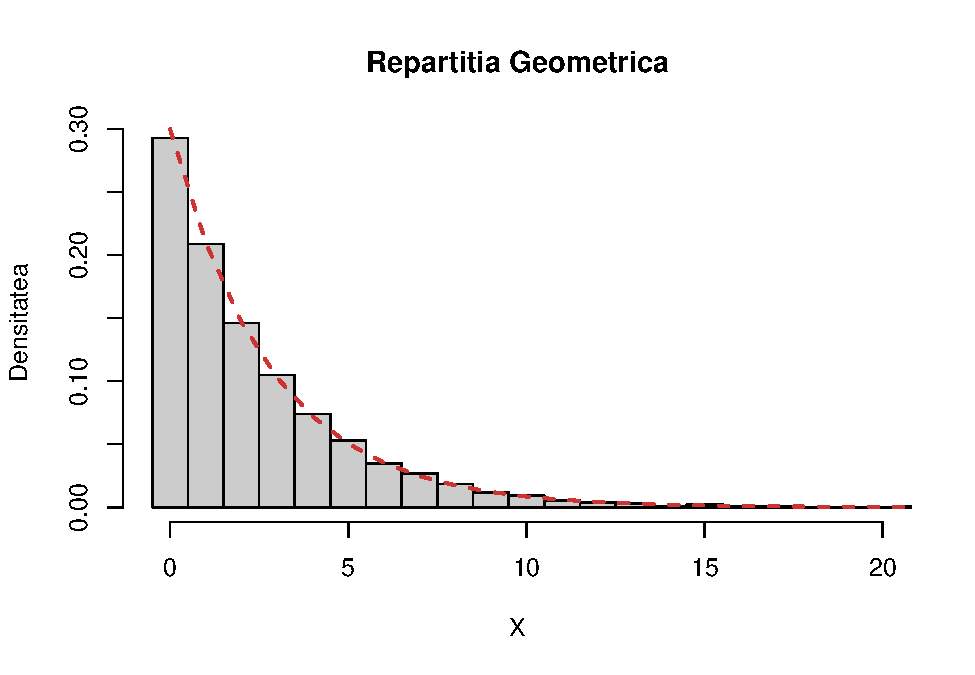
\includegraphics{Lab_4_files/figure-latex/unnamed-chunk-5-1} \end{center}

\section{Funcția de repartiție pentru variabile
aleatoare}\label{functia-de-repartitie-pentru-variabile-aleatoare}

\begin{rmdexercise}
Scrieți o funcție în \texttt{R} care să traseze graficul funcției de
repartitie a unei distribuții date. Verificați și documentația funcției
\texttt{ecdf}.
\end{rmdexercise}

Definim următoarea funcție:

\begin{Shaded}
\begin{Highlighting}[]
\NormalTok{cdfPlot =}\StringTok{ }\ControlFlowTok{function}\NormalTok{(dist, title, }\DataTypeTok{err =} \FloatTok{1e-10}\NormalTok{)\{}
  \CommentTok{# dist - repartitia discreta (sau discretizata)}
\NormalTok{  lp =}\StringTok{ }\KeywordTok{length}\NormalTok{(dist)}
  
  \ControlFlowTok{if}\NormalTok{ (}\KeywordTok{abs}\NormalTok{(}\KeywordTok{sum}\NormalTok{(dist)}\OperatorTok{-}\DecValTok{1}\NormalTok{)}\OperatorTok{>}\NormalTok{err }\OperatorTok{|}\StringTok{ }\KeywordTok{sum}\NormalTok{(dist}\OperatorTok{>=}\DecValTok{0}\NormalTok{)}\OperatorTok{!=}\NormalTok{lp)\{}
    \KeywordTok{stop}\NormalTok{(}\StringTok{"Eroare: vectorul de probabilitati nu formeaza o repartitie"}\NormalTok{)}
\NormalTok{  \}}\ControlFlowTok{else}\NormalTok{\{}
\NormalTok{    x =}\StringTok{ }\DecValTok{0}\OperatorTok{:}\NormalTok{(lp}\OperatorTok{-}\DecValTok{1}\NormalTok{) }\CommentTok{# ia valori in 1:lp}
\NormalTok{    cp =}\StringTok{ }\KeywordTok{cumsum}\NormalTok{(dist)}
    
    \KeywordTok{plot}\NormalTok{(x, cp, }\DataTypeTok{type =} \StringTok{"s"}\NormalTok{, }\DataTypeTok{lty =} \DecValTok{3}\NormalTok{, }
         \DataTypeTok{xlab =} \StringTok{"x"}\NormalTok{, }
         \DataTypeTok{ylab =} \StringTok{"F"}\NormalTok{, }
         \DataTypeTok{main =} \KeywordTok{paste}\NormalTok{(}\StringTok{"Functia de repartitie:"}\NormalTok{, title), }
         \DataTypeTok{ylim =} \KeywordTok{c}\NormalTok{(}\DecValTok{0}\NormalTok{,}\DecValTok{1}\NormalTok{), }
         \DataTypeTok{col =} \StringTok{"grey"}\NormalTok{,}
         \DataTypeTok{bty =} \StringTok{"n"}\NormalTok{)}
    \KeywordTok{abline}\NormalTok{(}\DataTypeTok{h =} \DecValTok{0}\NormalTok{, }\DataTypeTok{lty =} \DecValTok{2}\NormalTok{, }\DataTypeTok{col =} \StringTok{"grey"}\NormalTok{)}
    \KeywordTok{abline}\NormalTok{(}\DataTypeTok{h =} \DecValTok{1}\NormalTok{, }\DataTypeTok{lty =} \DecValTok{2}\NormalTok{, }\DataTypeTok{col =} \StringTok{"grey"}\NormalTok{)}
    \ControlFlowTok{for}\NormalTok{(i }\ControlFlowTok{in} \DecValTok{1}\OperatorTok{:}\NormalTok{(lp}\OperatorTok{-}\DecValTok{1}\NormalTok{))\{}
      \KeywordTok{lines}\NormalTok{(}\KeywordTok{c}\NormalTok{(x[i], x[i}\OperatorTok{+}\DecValTok{1}\NormalTok{]), }\KeywordTok{c}\NormalTok{(cp[i], cp[i]), }\DataTypeTok{lwd =} \DecValTok{2}\NormalTok{)}
\NormalTok{    \}}
    \KeywordTok{points}\NormalTok{(x,cp, }\DataTypeTok{col =} \StringTok{"black"}\NormalTok{, }\DataTypeTok{pch =} \DecValTok{20}\NormalTok{, }\DataTypeTok{cex =} \FloatTok{0.85}\NormalTok{)}
\NormalTok{  \}}
\NormalTok{\}}
\end{Highlighting}
\end{Shaded}

Pentru a testa această funcție să considerăm repartițiile discrete:

\begin{enumerate}
\def\labelenumi{\alph{enumi})}
\tightlist
\item
  Binomiala: \(\mathcal{B}(100, 0.3)\)
\end{enumerate}

\begin{Shaded}
\begin{Highlighting}[]
\KeywordTok{cdfPlot}\NormalTok{(}\DataTypeTok{dist =} \KeywordTok{dbinom}\NormalTok{(}\DecValTok{0}\OperatorTok{:}\DecValTok{100}\NormalTok{, }\DecValTok{100}\NormalTok{, }\FloatTok{0.3}\NormalTok{), }\DataTypeTok{title =} \StringTok{"B(100,0.3)"}\NormalTok{)}
\end{Highlighting}
\end{Shaded}

\begin{center}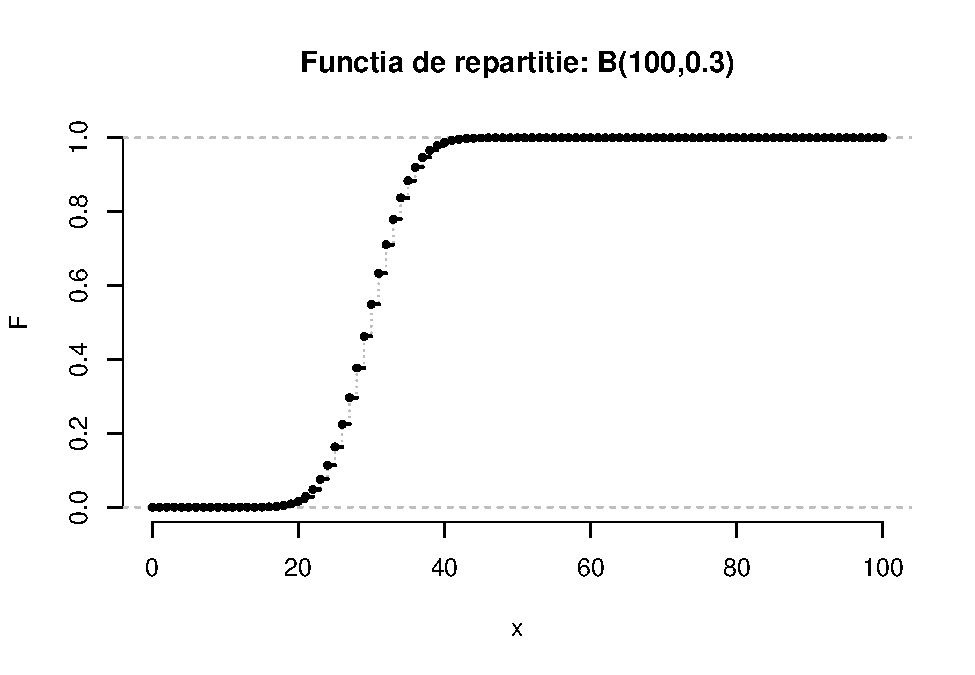
\includegraphics[width=0.8\linewidth]{Lab_4_files/figure-latex/unnamed-chunk-8-1} \end{center}

\begin{enumerate}
\def\labelenumi{\alph{enumi})}
\setcounter{enumi}{1}
\tightlist
\item
  Poisson: \(Pois(0.3)\) și \(Pois(5)\)
\end{enumerate}

\begin{Shaded}
\begin{Highlighting}[]
\KeywordTok{par}\NormalTok{(}\DataTypeTok{mfrow =} \KeywordTok{c}\NormalTok{(}\DecValTok{1}\NormalTok{, }\DecValTok{2}\NormalTok{))}

\KeywordTok{cdfPlot}\NormalTok{(}\DataTypeTok{dist =} \KeywordTok{dpois}\NormalTok{(}\DecValTok{0}\OperatorTok{:}\DecValTok{20}\NormalTok{, }\FloatTok{0.3}\NormalTok{), }\DataTypeTok{title =} \StringTok{"Pois(0.3)"}\NormalTok{)}
\KeywordTok{cdfPlot}\NormalTok{(}\DataTypeTok{dist =} \KeywordTok{dpois}\NormalTok{(}\DecValTok{0}\OperatorTok{:}\DecValTok{50}\NormalTok{, }\DecValTok{5}\NormalTok{), }\DataTypeTok{title =} \StringTok{"Pois(5)"}\NormalTok{)}
\end{Highlighting}
\end{Shaded}

\begin{center}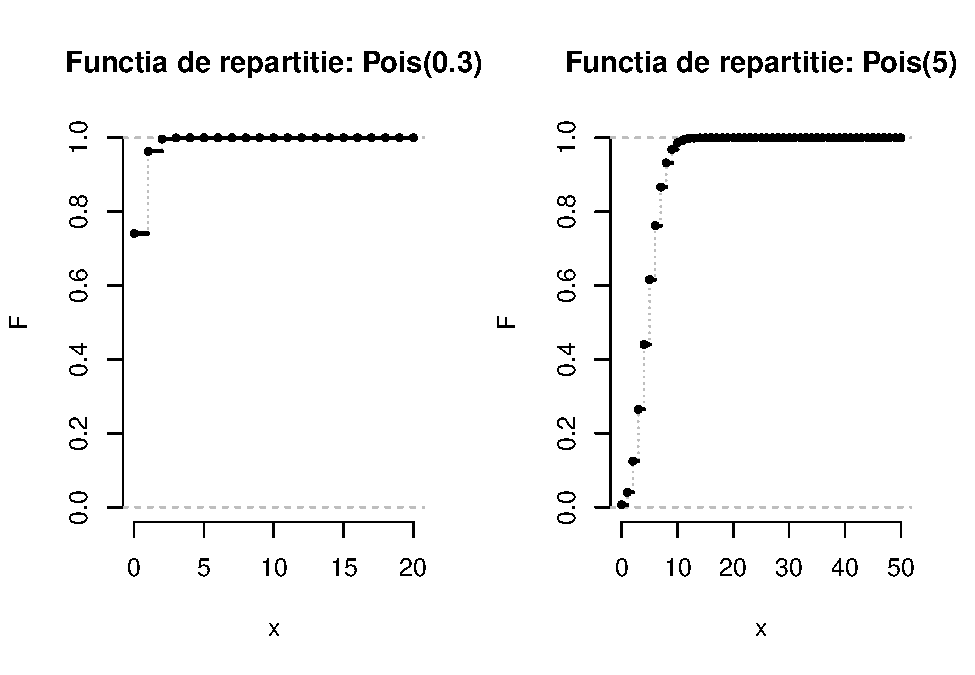
\includegraphics{Lab_4_files/figure-latex/unnamed-chunk-9-1} \end{center}

\begin{enumerate}
\def\labelenumi{\alph{enumi})}
\setcounter{enumi}{2}
\tightlist
\item
  Geometrica: \(Geom(0.3)\)
\end{enumerate}

\begin{Shaded}
\begin{Highlighting}[]
\KeywordTok{par}\NormalTok{(}\DataTypeTok{mfrow =} \KeywordTok{c}\NormalTok{(}\DecValTok{1}\NormalTok{,}\DecValTok{1}\NormalTok{))}
\KeywordTok{cdfPlot}\NormalTok{(}\DataTypeTok{dist =} \KeywordTok{dgeom}\NormalTok{(}\DecValTok{0}\OperatorTok{:}\DecValTok{100}\NormalTok{, }\FloatTok{0.3}\NormalTok{), }\DataTypeTok{title =} \StringTok{"Geom(0.3)"}\NormalTok{)}
\end{Highlighting}
\end{Shaded}

\begin{center}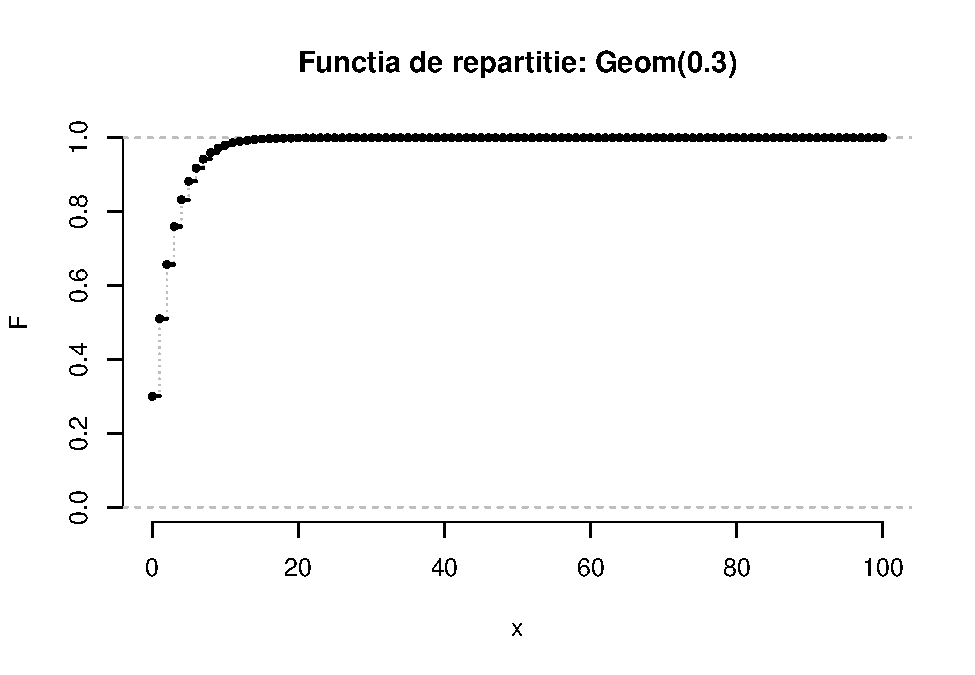
\includegraphics[width=0.8\linewidth]{Lab_4_files/figure-latex/unnamed-chunk-10-1} \end{center}

și repartiția continuă:

\begin{enumerate}
\def\labelenumi{\alph{enumi})}
\tightlist
\item
  Normala: \(\mathcal{N}(0,1)\)
\end{enumerate}

\begin{Shaded}
\begin{Highlighting}[]
\KeywordTok{cdfPlot}\NormalTok{(}\DataTypeTok{dist =} \KeywordTok{dnorm}\NormalTok{(}\KeywordTok{seq}\NormalTok{(}\OperatorTok{-}\DecValTok{5}\NormalTok{,}\DecValTok{5}\NormalTok{,}\FloatTok{0.01}\NormalTok{))}\OperatorTok{/}\DecValTok{100}\NormalTok{, }\DataTypeTok{title =} \StringTok{"N(0,1)"}\NormalTok{, }\DataTypeTok{err =} \FloatTok{1e-1}\NormalTok{)}
\end{Highlighting}
\end{Shaded}

\begin{center}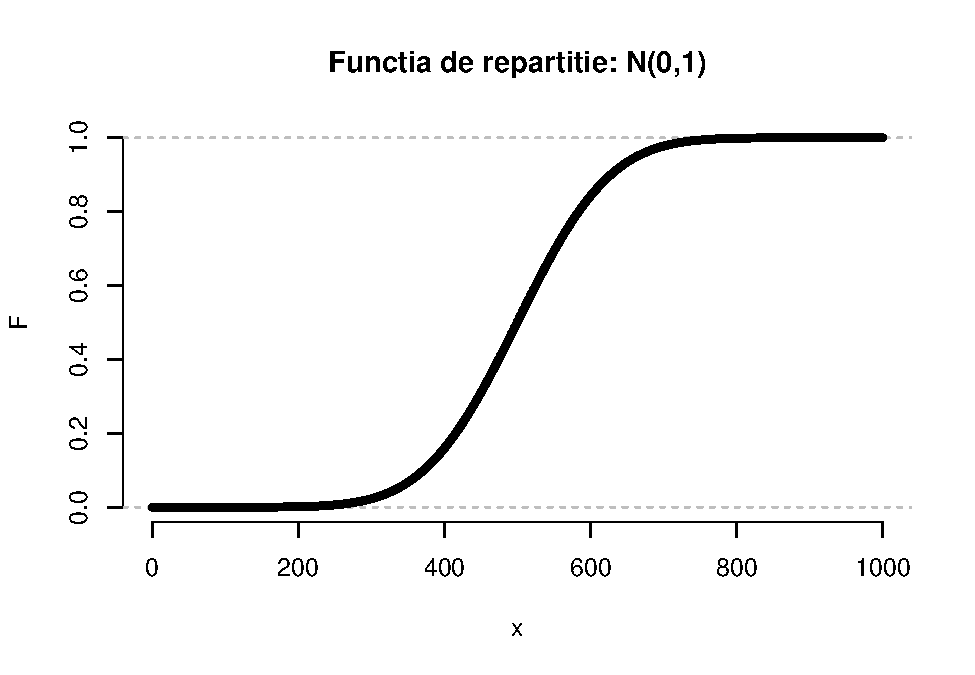
\includegraphics[width=0.8\linewidth]{Lab_4_files/figure-latex/unnamed-chunk-11-1} \end{center}

\section{Aproximarea Poisson și Normală a
Binomialei}\label{aproximarea-poisson-si-normala-a-binomialei}

\begin{rmdexercise}
Ilustrați grafic aproximarea Poisson și normală a repartiției binomiale.
\end{rmdexercise}

Scopul acestei probleme este de a ilustra grafic aproximarea legii
binomile cu ajutorul repartiției Poisson și a a normalei.

Pentru o v.a. \(X\) repartizată binomial de parametrii \(n\) și \(p\)
(\(q = 1-p\)) funcția de masă este

\[
f_{n,p}(k)=\mathbb{P}(X=k)=\binom{n}{k}p^k(1-p)^{n-k}
\]

iar funcția de repartiție este

\[
F_{n,p}(k) = \mathbb{P}(X\leq k) = \sum_{x=0}^{k}\binom{n}{x}p^x(1-p)^{n-x}.
\]

\subsection{Aproximarea Poisson}\label{aproximarea-poisson}

Dacă \(n\to\infty\) (\(n\) este mare) și \(p\to 0\) (\(p\) este mic,
evenimentele sunt rare) așa încât \(np\to\lambda\) atunci se poate
verifica cu ușurință că

\[
f_{n,p}(k)\approx f_{\lambda}(k)=e^{-\lambda}\frac{\lambda^k}{k!}.
\]

Mai exact, avem că dacă \(k\) este mic în comparație cu \(n\) atunci

\begin{align*}
  \binom{n}{k}p^k &= \frac{n(n-1)\cdots(n-k+1)}{k!}\left(\frac{\lambda}{n}\right)^k \\
                  &= 1\times\left(1-\frac{1}{n}\right)\times\cdots\times\left(1-\frac{k-1}{n}\right)\frac{\lambda^k}{k!}\\
                  &\approx \frac{\lambda^k}{k!}
\end{align*}

și

\[
  \log(1-p)^{n-k} = (n-k)\log\left(1-\frac{\lambda}{n}\right)\approx n\left(-\frac{\lambda}{n}\right)
\]

ceea ce conduce la \((1-p)^{n-k}\approx e^{-\lambda}\). Combinând cele
două aproximări obținem

\[
  \binom{n}{k}p^k(1-p)^{n-k} \approx \frac{\lambda^k}{k!}e^{-\lambda}.
\]

Pentru a ilustra acuratețea acestei aproximări vom folosi instrucțiunile
\texttt{R} \texttt{dbinom} și \texttt{dpois} care permit calcularea
funcțiilor de masă \(f_{n,p}(k)\) și \(f_{\lambda}(k)\).

\begin{Shaded}
\begin{Highlighting}[]
\NormalTok{AppBP <-}\StringTok{ }\ControlFlowTok{function}\NormalTok{(n,p,a,b)\{}
\NormalTok{    lambda <-}\StringTok{ }\NormalTok{n}\OperatorTok{*}\NormalTok{p}
\NormalTok{    x<-}\StringTok{ }\KeywordTok{matrix}\NormalTok{(}\KeywordTok{numeric}\NormalTok{((b}\OperatorTok{-}\NormalTok{a}\OperatorTok{+}\DecValTok{1}\NormalTok{)}\OperatorTok{*}\DecValTok{3}\NormalTok{),}\DataTypeTok{ncol=}\DecValTok{3}\NormalTok{,}
               \DataTypeTok{dimnames =} \KeywordTok{list}\NormalTok{(a}\OperatorTok{:}\NormalTok{b,}\KeywordTok{c}\NormalTok{(}\StringTok{"Binomiala"}\NormalTok{,}\StringTok{"Poisson"}\NormalTok{,}\StringTok{"Eroarea Absoluta"}\NormalTok{)))}
\NormalTok{    x[,}\DecValTok{1}\NormalTok{]<-}\KeywordTok{dbinom}\NormalTok{(a}\OperatorTok{:}\NormalTok{b,n,p)}
\NormalTok{    x[,}\DecValTok{2}\NormalTok{]<-}\KeywordTok{dpois}\NormalTok{(a}\OperatorTok{:}\NormalTok{b,lambda)}
\NormalTok{    x[,}\DecValTok{3}\NormalTok{]<-}\KeywordTok{abs}\NormalTok{(x[,}\DecValTok{1}\NormalTok{]}\OperatorTok{-}\NormalTok{x[,}\DecValTok{2}\NormalTok{])}
\NormalTok{    error <-}\StringTok{ }\KeywordTok{max}\NormalTok{(}\KeywordTok{abs}\NormalTok{(x[,}\DecValTok{3}\NormalTok{]))}
    
    \KeywordTok{return}\NormalTok{(}\KeywordTok{list}\NormalTok{(}\DataTypeTok{x =} \KeywordTok{as.data.frame}\NormalTok{(x), }\DataTypeTok{error =}\NormalTok{ error, }\DataTypeTok{param =} \KeywordTok{c}\NormalTok{(n, p, lambda)))}
\NormalTok{\}}

\CommentTok{# Functie care ilustreaza aproximarea Binomial vs. Poisson}

\NormalTok{pl <-}\StringTok{ }\ControlFlowTok{function}\NormalTok{(n,p,a,b)\{}
\NormalTok{    clr<-}\KeywordTok{c}\NormalTok{(}\StringTok{"#E69F00"}\NormalTok{, }\StringTok{"#56B4E9"}\NormalTok{)}\CommentTok{# culori}
\NormalTok{    lambda <-}\StringTok{ }\NormalTok{n}\OperatorTok{*}\NormalTok{p}
\NormalTok{    mx <-}\StringTok{ }\KeywordTok{max}\NormalTok{(}\KeywordTok{dbinom}\NormalTok{(a}\OperatorTok{:}\NormalTok{b,n,p))}
    \KeywordTok{plot}\NormalTok{(}\KeywordTok{c}\NormalTok{(a}\OperatorTok{:}\NormalTok{b,a}\OperatorTok{:}\NormalTok{b), }\KeywordTok{c}\NormalTok{(}\KeywordTok{dbinom}\NormalTok{(a}\OperatorTok{:}\NormalTok{b,n,p), }\KeywordTok{dpois}\NormalTok{(a}\OperatorTok{:}\NormalTok{b,lambda)), }\DataTypeTok{type=}\StringTok{"n"}\NormalTok{, }
         \DataTypeTok{main =} \KeywordTok{paste}\NormalTok{(}\StringTok{"Approx. Poisson pentru binomiala}\CharTok{\textbackslash{}n}\StringTok{ n="}\NormalTok{, }
\NormalTok{                      n, }\StringTok{", p = "}\NormalTok{, p, }\StringTok{", lambda = "}\NormalTok{,lambda), }
         \DataTypeTok{ylab =} \StringTok{"Probabilitatea"}\NormalTok{, }\DataTypeTok{xlab=}\StringTok{"x"}\NormalTok{,}
         \DataTypeTok{bty =} \StringTok{"n"}\NormalTok{)}
    \KeywordTok{points}\NormalTok{((a}\OperatorTok{:}\NormalTok{b)}\OperatorTok{-}\NormalTok{.}\DecValTok{15}\NormalTok{, }\KeywordTok{dbinom}\NormalTok{(a}\OperatorTok{:}\NormalTok{b,n,p), }\DataTypeTok{type =} \StringTok{"h"}\NormalTok{,}\DataTypeTok{col =}\NormalTok{ clr[}\DecValTok{1}\NormalTok{], }\DataTypeTok{lwd =} \DecValTok{8}\NormalTok{)}
    \KeywordTok{points}\NormalTok{((a}\OperatorTok{:}\NormalTok{b)}\OperatorTok{+}\NormalTok{.}\DecValTok{15}\NormalTok{, }\KeywordTok{dpois}\NormalTok{(a}\OperatorTok{:}\NormalTok{b,lambda), }\DataTypeTok{type =} \StringTok{"h"}\NormalTok{,}\DataTypeTok{col =}\NormalTok{ clr[}\DecValTok{2}\NormalTok{], }\DataTypeTok{lwd =} \DecValTok{8}\NormalTok{)}
    \KeywordTok{legend}\NormalTok{(b}\OperatorTok{-}\NormalTok{b}\OperatorTok{/}\DecValTok{2}\NormalTok{, mx, }\DataTypeTok{legend =} \KeywordTok{c}\NormalTok{(}\KeywordTok{paste0}\NormalTok{(}\StringTok{"Binomiala("}\NormalTok{,n,}\StringTok{","}\NormalTok{,p,}\StringTok{")"}\NormalTok{),}
                               \KeywordTok{paste0}\NormalTok{(}\StringTok{"Poisson("}\NormalTok{,lambda,}\StringTok{")"}\NormalTok{)), }
           \DataTypeTok{fill =}\NormalTok{ clr, }\DataTypeTok{bg=}\StringTok{"white"}\NormalTok{,}
           \DataTypeTok{bty =} \StringTok{"n"}\NormalTok{)}
\NormalTok{\}}
\end{Highlighting}
\end{Shaded}

Pentru setul de parametrii \(n=20\) și \(p=0.3\) avem următorul tabel și
următoarea figură

\begin{longtable}[]{@{}cccc@{}}
\caption{Aproximarea Poisson la binomiala n = 20 p = 0.3 lambda = 6 .
Eroarea (Diferenta in valoare absoluta maxima) = 0.03102
.}\tabularnewline
\toprule
k & Binomiala & Poisson & Eroarea Absoluta\tabularnewline
\midrule
\endfirsthead
\toprule
k & Binomiala & Poisson & Eroarea Absoluta\tabularnewline
\midrule
\endhead
1 & 0.0068393 & 0.0148725 & 0.0080332\tabularnewline
2 & 0.0278459 & 0.0446175 & 0.0167717\tabularnewline
3 & 0.0716037 & 0.0892351 & 0.0176314\tabularnewline
4 & 0.1304210 & 0.1338526 & 0.0034316\tabularnewline
5 & 0.1788631 & 0.1606231 & 0.0182399\tabularnewline
6 & 0.1916390 & 0.1606231 & 0.0310158\tabularnewline
7 & 0.1642620 & 0.1376770 & 0.0265850\tabularnewline
8 & 0.1143967 & 0.1032577 & 0.0111390\tabularnewline
9 & 0.0653696 & 0.0688385 & 0.0034689\tabularnewline
10 & 0.0308171 & 0.0413031 & 0.0104860\tabularnewline
11 & 0.0120067 & 0.0225290 & 0.0105223\tabularnewline
12 & 0.0038593 & 0.0112645 & 0.0074052\tabularnewline
13 & 0.0010178 & 0.0051990 & 0.0041812\tabularnewline
14 & 0.0002181 & 0.0022281 & 0.0020100\tabularnewline
15 & 0.0000374 & 0.0008913 & 0.0008539\tabularnewline
\bottomrule
\end{longtable}

\begin{center}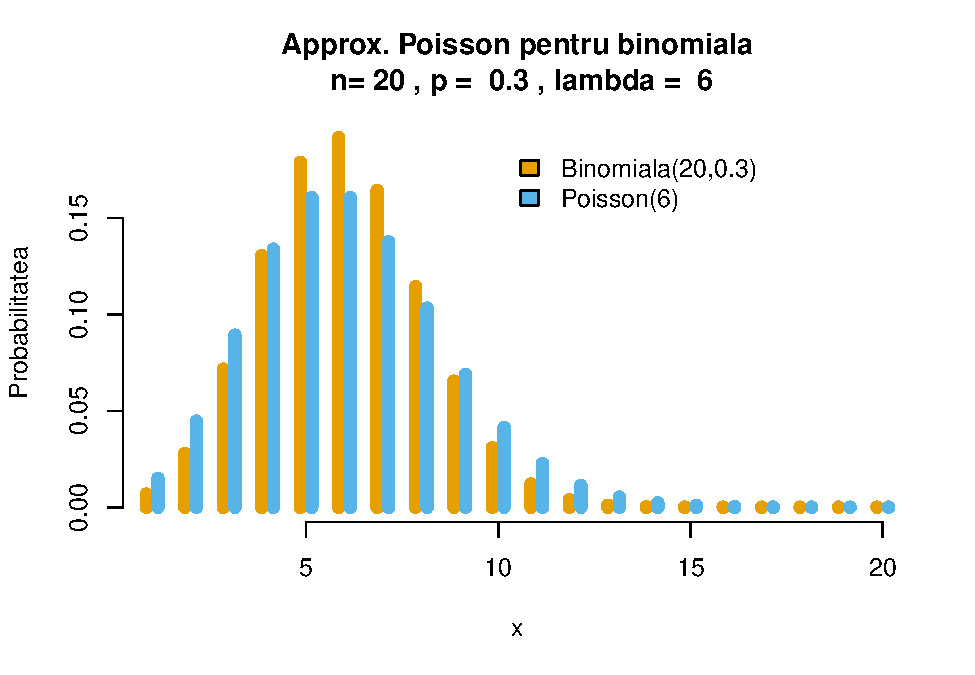
\includegraphics{Lab_4_files/figure-latex/unnamed-chunk-15-1} \end{center}

iar pentru parametrii \(n=100\) și \(p=0.01\) obținem

\begin{longtable}[]{@{}cccc@{}}
\caption{Aproximarea Poisson la binomiala n = 100 p = 0.01 lambda = 1 .
Eroarea (Diferenta in valoare absoluta maxima) = 0.00185
.}\tabularnewline
\toprule
k & Binomiala & Poisson & Eroarea Absoluta\tabularnewline
\midrule
\endfirsthead
\toprule
k & Binomiala & Poisson & Eroarea Absoluta\tabularnewline
\midrule
\endhead
1 & 0.3697296 & 0.3678794 & 0.0018502\tabularnewline
2 & 0.1848648 & 0.1839397 & 0.0009251\tabularnewline
3 & 0.0609992 & 0.0613132 & 0.0003141\tabularnewline
4 & 0.0149417 & 0.0153283 & 0.0003866\tabularnewline
5 & 0.0028978 & 0.0030657 & 0.0001679\tabularnewline
6 & 0.0004635 & 0.0005109 & 0.0000475\tabularnewline
7 & 0.0000629 & 0.0000730 & 0.0000101\tabularnewline
8 & 0.0000074 & 0.0000091 & 0.0000017\tabularnewline
9 & 0.0000008 & 0.0000010 & 0.0000003\tabularnewline
10 & 0.0000001 & 0.0000001 & 0.0000000\tabularnewline
\bottomrule
\end{longtable}

\begin{center}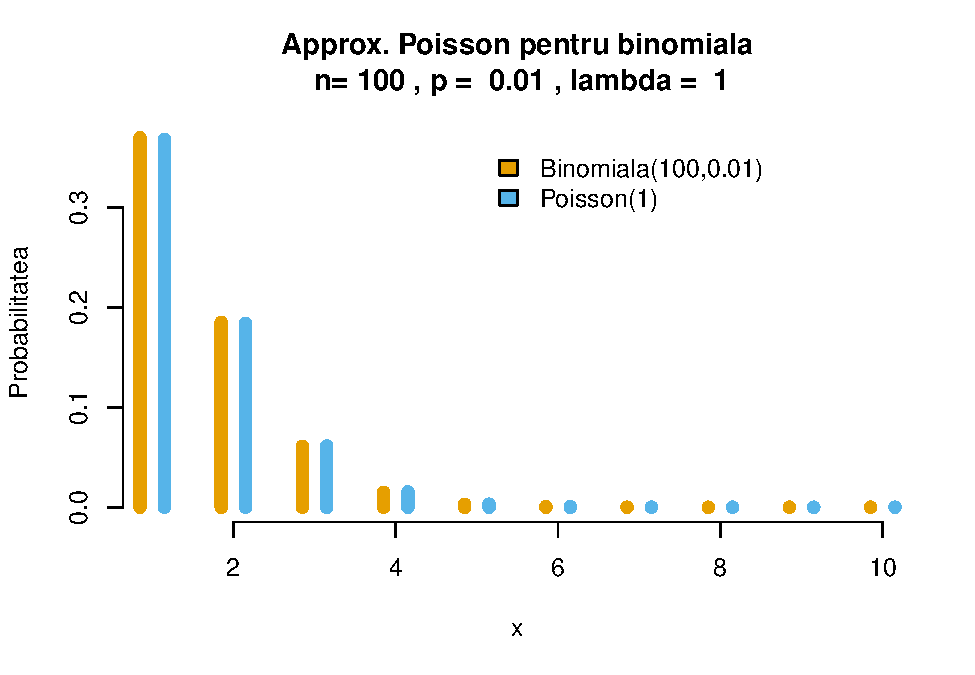
\includegraphics{Lab_4_files/figure-latex/unnamed-chunk-17-1} \end{center}

Pentru funcția de repartiție \(F_{n,p}(k)\), folosidn aproximarea
Poisson avem că

\[
F_{n,p}(k) \approx F_{\lambda}(k)=\sum_{x=0}^{k}e^{-\lambda}\frac{\lambda^x}{x!}.
\]

\subsection{Aproximarea Normală}\label{aproximarea-normala}

Să considerăm repartiția binomială \(\mathcal{B}(n, p)\) pentru
\(p = 0.3\) și \(n\in\{20, 50, 100, 150, 200\}\) și să trasăm
histogramele variabilelor aleatoare care au aceste repartiții (\(X_n\))
precum și a variabilelor standardizate
\(Z_n = \frac{X_n-np}{\sqrt{npq}}\).

\begin{center}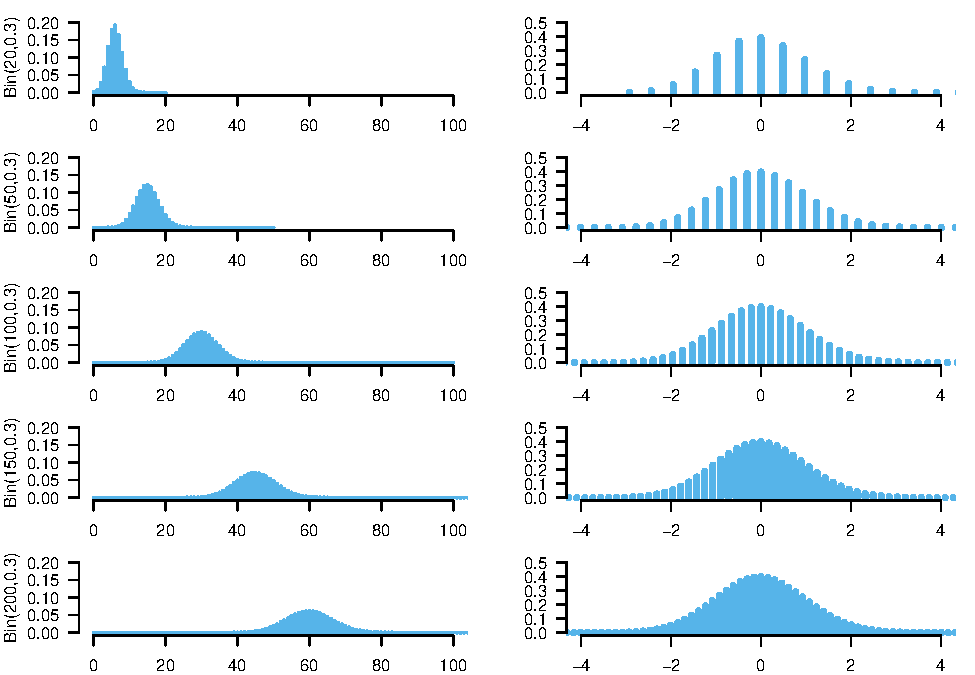
\includegraphics{Lab_4_files/figure-latex/unnamed-chunk-18-1} \end{center}

Observăm, pentru graficele din partea stângă, că valoarea maximă se
atinge în jurul punctului \(n\times 0.3\) pentru fiecare grafic în
parte. De asemenea se observă că odată cu creșterea lui \(n\) crește și
gradul de împrăștiere, cu alte cuvinte crește și abaterea standard
(\(\sigma_n = \sqrt{npq}\)).

Pe de altă parte putem remarca că figurile din partea dreaptă au o formă
simetrică, de tip \emph{clopot}, concentrate în jurul lui \(0\), fiind
translatate în origine și scalate pentru a avea o varianță egală cu
\(1\). \href{https://en.wikipedia.org/wiki/Abraham_de_Moivre}{Abraham de
Moivre}\footnote{de Moivre, A. (1756). \emph{The Doctrine of Chances:
  or, A Method of Calculating the Probabilities of Events in Play}
  (Third ed.). New York: Chelsea.} a justificat acest efect (pentru
\(p=0.5\)) încă din 1756 observând că raportul

\[
  \frac{f_{n,p}(k)}{f_{n,p}(k-1)} = \frac{\frac{n!}{k!(n-k)!}p^kq^{n-k}}{\frac{n!}{(k-1)!(n-k+1)!}p^{k+1}q^{n-k+1}} = \frac{(n-k+1)p}{kq}
\]

pentru \(k = 1,2,\ldots,n\). Astfel \(f_{n,p}(k)\geq f_{n,p}(k-1)\) dacă
și numai dacă \((n+1)p\geq k\) de unde, pentru \(n\) fixat, deducem că
\(f_{n,p}(k)\) atinge valoarea maximă pentru
\(k_{\max} = \lfloor{(n+1)p\rfloor}\approx np\) (acesta este motivul
pentru care fiecare grafic din partea stângă are vârful în jurul
punctului \(np\)).

Să observăm ce se întâmplă în jurul lui \(k_{\max}\). Avem

\[
\frac{f_{n,p}(k_{\max}+i)}{f_{n,p}(k_{\max}+i-1)} = \frac{(n-k_{\max}-i+1)p}{(k_{\max}+i)q}\approx \frac{(nq-i)p}{(np+i)q} = \frac{1-\frac{i}{nq}}{1+\frac{i}{np}}
\]

și cum (folosind relația \(\log(1+x)\approx x\), pentru \(x\) în jurul
lui \(0\))

\[
\log\left(1-\frac{i}{nq}\right) - \log\left(1+\frac{i}{np}\right) \approx -\frac{i}{nq}-\frac{i}{np} = -\frac{i}{npq}
\]

deducem, pentru \(m\geq 1\) și \(k_{\max}+m\leq n\), că

\begin{align*}
  \log\frac{f_{n,p}(k_{\max}+m)}{f_{n,p}(k_{\max})} &= \log\left(\frac{f_{n,p}(k_{\max}+1)}{f_{n,p}(k_{\max})}\times \frac{f_{n,p}(k_{\max}+2)}{f_{n,p}(k_{\max}+1)}\times\cdots\times\frac{f_{n,p}(k_{\max}+m)}{f_{n,p}(k_{\max}+m-1)}\right)\\
  &= \log\frac{f_{n,p}(k_{\max}+1)}{f_{n,p}(k_{\max})}+ \log\frac{f_{n,p}(k_{\max}+2)}{f_{n,p}(k_{\max}+1)}+\cdots+\log\frac{f_{n,p}(k_{\max}+m)}{f_{n,p}(k_{\max}+m-1)}\\
  &\approx \frac{-1-2-\cdots-m}{npq} = -\frac{1}{2}\frac{m^2}{npq}.
\end{align*}

Sumarizând avem, pentru \(m\) nu foarte mare,

\[
  \mathbb{P}(X=k_{\max}+m)\approx f_{n,p}(k_{\max})e^{-\frac{1}{2}\frac{m^2}{npq}}.
\]

Folosind formula lui
\href{https://en.wikipedia.org/wiki/Stirling\%27s_approximation}{Stirling}\footnote{A
  se vedea cartea lui Feller, W. (1968). \emph{An Introduction to
  Probability Theory and Its Applications} (third ed.), Volume 1. New
  York: Wiley. pag. 52-53 pentru o derivare a formulei lui Stirling.}

\[
  n!\approx \sqrt{2\pi}n^{n+\frac{1}{2}}e^{-n}
\]

pentru \(k = k_{\max}\approx np\), avem

\[
f_{n,p}(k)\approx \frac{1}{\sqrt{2\pi}}\frac{n^{n+\frac{1}{2}}}{(np)^{np+\frac{1}{2}}(nq)^{nq+\frac{1}{2}}}p^{np}q^{nq}= \frac{1}{\sqrt{2\pi npq}}.
\]

Astfel aproximarea de Moivre devine

\[
  \mathbb{P}(X=k_{\max}+m)\approx \frac{1}{\sqrt{2\pi npq}}e^{-\frac{1}{2}\frac{m^2}{npq}}
\]

și scriind \(k\) pentru \(k_{\max}+m\) și înlocuind \(k_{\max}\) cu
\(np\) obținem

\[
  \mathbb{P}(X=k)\approx \frac{1}{\sqrt{2\pi npq}}e^{-\frac{1}{2}\frac{(k-np)^2}{npq}} = \frac{1}{\sigma_n\sqrt{2\pi}}e^{-\frac{1}{2}\left(\frac{k-np}{\sigma_n}\right)^2}.
\]

Astfel \(mathbb{P}(X=k)\) este aproximativ egală cu aria de sub curba

\[
  f(x) = \frac{1}{\sigma_n\sqrt{2\pi}}e^{-\frac{1}{2}\left(\frac{x-np}{\sigma_n}\right)^2}
\] pe intervalul \(k-\frac{1}{2}\leq x\leq k+\frac{1}{2}\).

În mod similar, pentru \(0\leq a< b\leq n\), avem

\[
  \mathbb{P}(a\leq X\leq b) = \sum_{k=a}^{b}f_{n,p}(k) \approx \sum_{k=a}^{k=b}\int_{k+\frac{1}{2}}^{k-\frac{1}{2}}f(x)\,dx = \int_{a}^{b}f(x)\,dx
\]

de unde prin schimbarea de variabilă \(y = \frac{x-np}{\sigma_n}\)
obținem

\[
  \mathbb{P}(a\leq X\leq b)\approx \frac{1}{\sqrt{2\pi}}\int_{\alpha}^{\beta}e^{-\frac{y^2}{2}}\,dy = \Phi(\beta) - \Phi(\alpha)
\]

unde \(\alpha = \frac{a-np-\frac{1}{2}}{\sigma_n}\),
\(\beta = = \frac{b-np+\frac{1}{2}}{\sigma_n}\) și
\(\Phi(x)=\frac{1}{\sqrt{2\pi}}\int_{-\infty}^{x}e^{-\frac{y^2}{2}}\,dy\).

Aplicând rezultatele de mai sus, în cele ce urmează vom considera două
aproximări pentru funcția de repartiție \(F_{n,p}(k)\):

\begin{enumerate}
\def\labelenumi{\alph{enumi})}
\tightlist
\item
  aproximarea normală
\end{enumerate}

\[
F_{n,p}(k) \approx \Phi\left(\frac{k-np}{\sqrt{np(1-p)}}\right).
\]

\begin{enumerate}
\def\labelenumi{\alph{enumi})}
\setcounter{enumi}{1}
\tightlist
\item
  aproximarea normală cu coeficient de corecție de continuitate
\end{enumerate}

\[
F_{n,p}(k) \approx \Phi\left(\frac{k+0.5-np}{\sqrt{np(1-p)}}\right).
\]

În practică această ultimă aproximare se aplică atunci când atât
\(np\geq 5\) cât și \(n(1-p)\geq 5\).

Următorul cod crează o funcție care calculează cele trei aproximări
pentru funcția de repartiție binomială

\begin{Shaded}
\begin{Highlighting}[]
\NormalTok{appBNP <-}\StringTok{ }\ControlFlowTok{function}\NormalTok{(n, p, }\DataTypeTok{R =} \DecValTok{1000}\NormalTok{, }\DataTypeTok{k =} \DecValTok{6}\NormalTok{) \{}
\NormalTok{  trueval <-}\StringTok{ }\KeywordTok{pbinom}\NormalTok{(k, n, p) }\CommentTok{# adevarata valoare a functiei de repartitie in k}
\NormalTok{  prob.zcc <-}\StringTok{ }\NormalTok{prob.zncc <-}\StringTok{ }\NormalTok{prob.pois <-}\StringTok{ }\OtherTok{NULL}  \CommentTok{# initializare}
\NormalTok{  q =}\StringTok{ }\DecValTok{1}\OperatorTok{-}\NormalTok{p}
  \ControlFlowTok{for}\NormalTok{ (i }\ControlFlowTok{in} \DecValTok{1}\OperatorTok{:}\NormalTok{R) \{}\CommentTok{# repetam procesul de R ori }
\NormalTok{    x =}\StringTok{ }\KeywordTok{rnorm}\NormalTok{(n, n }\OperatorTok{*}\StringTok{ }\NormalTok{p, }\KeywordTok{sqrt}\NormalTok{(n }\OperatorTok{*}\StringTok{ }\NormalTok{p }\OperatorTok{*}\StringTok{ }\NormalTok{q)) }\CommentTok{# generare n v.a. normale de medie np }
\NormalTok{    z.cc =}\StringTok{ }\NormalTok{((k }\OperatorTok{+}\StringTok{ }\NormalTok{.}\DecValTok{5}\NormalTok{) }\OperatorTok{-}\StringTok{ }\KeywordTok{mean}\NormalTok{(x))}\OperatorTok{/}\KeywordTok{sd}\NormalTok{(x) }\CommentTok{# cu coeficient de corectie}
\NormalTok{    prob.zcc[i] =}\StringTok{ }\KeywordTok{pnorm}\NormalTok{(z.cc)}
\NormalTok{    z.ncc =}\StringTok{ }\NormalTok{(k }\OperatorTok{-}\StringTok{ }\KeywordTok{mean}\NormalTok{(x))}\OperatorTok{/}\KeywordTok{sd}\NormalTok{(x) }\CommentTok{# fara coeficient de corectie}
\NormalTok{    prob.zncc[i] =}\StringTok{ }\KeywordTok{pnorm}\NormalTok{(z.ncc)    }
\NormalTok{    y =}\StringTok{ }\KeywordTok{rpois}\NormalTok{(n, n }\OperatorTok{*}\StringTok{ }\NormalTok{p)}
\NormalTok{    prob.pois[i] =}\StringTok{ }\KeywordTok{length}\NormalTok{(y[y }\OperatorTok{<=}\StringTok{ }\NormalTok{k])}\OperatorTok{/}\NormalTok{n }\CommentTok{# aproximate Poisson}
\NormalTok{  \}}
  \KeywordTok{list}\NormalTok{(}\DataTypeTok{prob.zcc =}\NormalTok{ prob.zcc, }\DataTypeTok{prob.zncc =}\NormalTok{ prob.zncc, }
       \DataTypeTok{prob.pois =}\NormalTok{ prob.pois, }\DataTypeTok{trueval =}\NormalTok{ trueval)}
\NormalTok{\}}
\end{Highlighting}
\end{Shaded}

Avem următoarea ilustrație grafică a diferitelor metode de aproximare

\begin{Shaded}
\begin{Highlighting}[]
\CommentTok{# Plot}
\NormalTok{R <-}\StringTok{ }\DecValTok{1000}
\KeywordTok{set.seed}\NormalTok{(}\DecValTok{10}\NormalTok{)}
\NormalTok{out <-}\StringTok{ }\KeywordTok{appBNP}\NormalTok{(}\DataTypeTok{n =} \DecValTok{100}\NormalTok{, }\DataTypeTok{p =}\NormalTok{ .}\DecValTok{01}\NormalTok{, }\DataTypeTok{k =} \DecValTok{2}\NormalTok{, }\DataTypeTok{R =} \DecValTok{1000}\NormalTok{)}

\KeywordTok{plot}\NormalTok{(}\DecValTok{1}\OperatorTok{:}\NormalTok{R, out}\OperatorTok{$}\NormalTok{prob.pois, }\DataTypeTok{type =} \StringTok{"l"}\NormalTok{, }\DataTypeTok{col =} \StringTok{"#E69F00"}\NormalTok{, }\DataTypeTok{xlab =} \StringTok{"Numar repetari"}\NormalTok{, }
     \DataTypeTok{main =} \KeywordTok{expression}\NormalTok{(}\KeywordTok{paste}\NormalTok{(}\StringTok{"Probabilitatile simulate: "}\NormalTok{, }
\NormalTok{                             n}\OperatorTok{==}\DecValTok{100}\NormalTok{, }\StringTok{", "}\NormalTok{, p}\OperatorTok{==}\FloatTok{0.01}\NormalTok{, }\DataTypeTok{sep=}\StringTok{""}\NormalTok{)),}
     \DataTypeTok{ylab =} \StringTok{"Probabilitatea"}\NormalTok{, }\DataTypeTok{ylim =} \KeywordTok{c}\NormalTok{(.}\DecValTok{7}\NormalTok{, .}\DecValTok{97}\NormalTok{),}
     \DataTypeTok{bty =} \StringTok{"n"}\NormalTok{)}
\KeywordTok{abline}\NormalTok{(}\DataTypeTok{h =}\NormalTok{ out}\OperatorTok{$}\NormalTok{trueval, }\DataTypeTok{col=}\StringTok{"black"}\NormalTok{, }\DataTypeTok{lty=}\DecValTok{2}\NormalTok{, }\DataTypeTok{lwd=}\DecValTok{2}\NormalTok{)}
\KeywordTok{lines}\NormalTok{(}\DecValTok{1}\OperatorTok{:}\NormalTok{R, out}\OperatorTok{$}\NormalTok{prob.zcc, }\DataTypeTok{lty =} \DecValTok{1}\NormalTok{, }\DataTypeTok{col =} \StringTok{"#56B4E9"}\NormalTok{)}
\KeywordTok{lines}\NormalTok{(}\DecValTok{1}\OperatorTok{:}\NormalTok{R, out}\OperatorTok{$}\NormalTok{prob.zncc, }\DataTypeTok{lty =} \DecValTok{1}\NormalTok{, }\DataTypeTok{col =} \StringTok{"gray80"}\NormalTok{)}
\KeywordTok{legend}\NormalTok{(}\StringTok{"bottomleft"}\NormalTok{, }\KeywordTok{c}\NormalTok{(}\StringTok{"Poisson"}\NormalTok{, }\StringTok{"Normala (cu factor corectie)"}\NormalTok{, }
                       \StringTok{"Normala (fara factor corectie)"}\NormalTok{),}
       \DataTypeTok{lty =} \KeywordTok{c}\NormalTok{(}\DecValTok{1}\NormalTok{), }\DataTypeTok{col =} \KeywordTok{c}\NormalTok{(}\StringTok{"#E69F00"}\NormalTok{, }\StringTok{"#56B4E9"}\NormalTok{, }\StringTok{"gray80"}\NormalTok{),}
       \DataTypeTok{bty =} \StringTok{"n"}\NormalTok{)}
\end{Highlighting}
\end{Shaded}

\begin{center}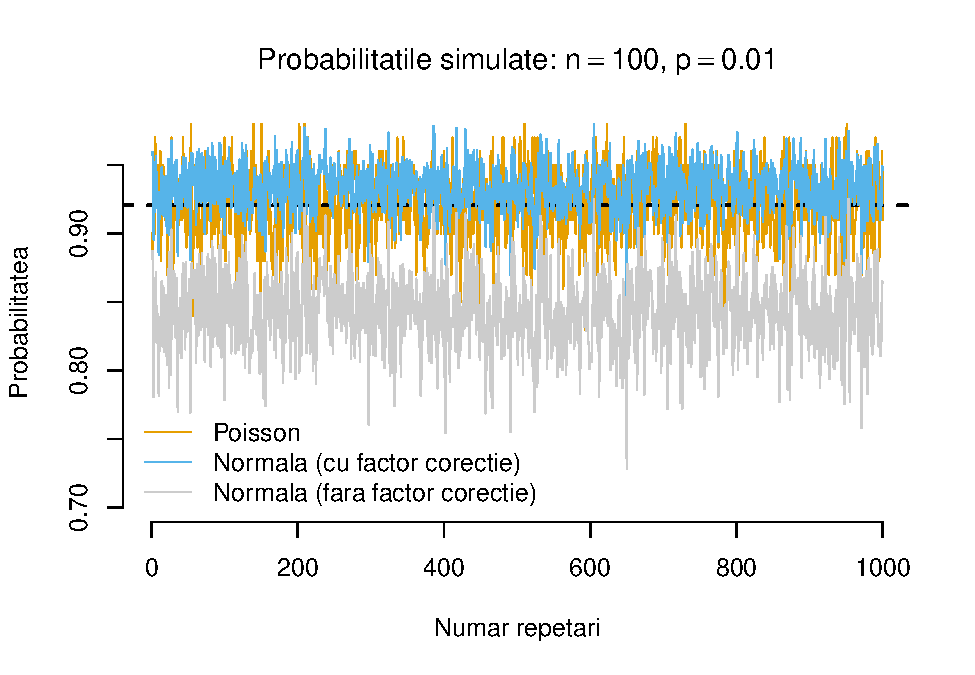
\includegraphics{Lab_4_files/figure-latex/unnamed-chunk-20-1} \end{center}

Avem și următorul \texttt{boxplot} (discuție ce reprezintă un boxplot)
care ne permite să evidențiem care dintre aproximări este mai bună
pentru valorile selectate

\begin{Shaded}
\begin{Highlighting}[]

\CommentTok{# n = 200}
\KeywordTok{set.seed}\NormalTok{(}\DecValTok{10}\NormalTok{)}
\NormalTok{out <-}\StringTok{ }\KeywordTok{appBNP}\NormalTok{(}\DataTypeTok{n =} \DecValTok{100}\NormalTok{, }\DataTypeTok{p =}\NormalTok{ .}\DecValTok{01}\NormalTok{, }\DataTypeTok{k =} \DecValTok{2}\NormalTok{, }\DataTypeTok{R =} \DecValTok{1000}\NormalTok{)}

\KeywordTok{boxplot}\NormalTok{(out}\OperatorTok{$}\NormalTok{prob.pois, }\DataTypeTok{boxwex =} \FloatTok{0.25}\NormalTok{, }\DataTypeTok{xlim =} \KeywordTok{c}\NormalTok{(}\FloatTok{0.5}\NormalTok{, }\FloatTok{1.5}\NormalTok{),}
        \DataTypeTok{col =} \StringTok{"#E69F00"}\NormalTok{,}
        \DataTypeTok{main =} \KeywordTok{expression}\NormalTok{(}\KeywordTok{paste}\NormalTok{(}\StringTok{"Aproximarea Binomialei: "}\NormalTok{, }
\NormalTok{                                n}\OperatorTok{==}\DecValTok{100}\NormalTok{, }\StringTok{", "}\NormalTok{, p}\OperatorTok{==}\FloatTok{0.01}\NormalTok{, }\DataTypeTok{sep=}\StringTok{""}\NormalTok{)),}
        \DataTypeTok{ylab =} \StringTok{"Probablitatea"}\NormalTok{, }
        \DataTypeTok{ylim =} \KeywordTok{c}\NormalTok{(out}\OperatorTok{$}\NormalTok{trueval }\OperatorTok{-}\StringTok{ }\FloatTok{0.1}\NormalTok{, out}\OperatorTok{$}\NormalTok{trueval }\OperatorTok{+}\StringTok{ }\FloatTok{0.15}\NormalTok{), }
        \DataTypeTok{bty =} \StringTok{"n"}\NormalTok{)}
\KeywordTok{boxplot}\NormalTok{(out}\OperatorTok{$}\NormalTok{prob.zcc, }\DataTypeTok{boxwex =} \FloatTok{0.25}\NormalTok{, }\DataTypeTok{at =} \DecValTok{1}\OperatorTok{:}\DecValTok{1} \OperatorTok{-}\StringTok{ }\FloatTok{0.2}\NormalTok{, }\DataTypeTok{add =}\NormalTok{ T,}
        \DataTypeTok{col =} \StringTok{"#56B4E9"}\NormalTok{)}
\KeywordTok{boxplot}\NormalTok{(out}\OperatorTok{$}\NormalTok{prob.zncc, }\DataTypeTok{boxwex =} \FloatTok{0.25}\NormalTok{, }\DataTypeTok{at =} \DecValTok{1}\OperatorTok{:}\DecValTok{1} \OperatorTok{+}\StringTok{ }\FloatTok{0.2}\NormalTok{, }\DataTypeTok{add =}\NormalTok{ T,}
        \DataTypeTok{col =} \StringTok{"gray80"}\NormalTok{ )}
\KeywordTok{abline}\NormalTok{(}\DataTypeTok{h =}\NormalTok{ out}\OperatorTok{$}\NormalTok{trueval, }\DataTypeTok{col =} \StringTok{"red"}\NormalTok{, }\DataTypeTok{lty=}\DecValTok{2}\NormalTok{)}
\KeywordTok{legend}\NormalTok{(}\StringTok{"topleft"}\NormalTok{, }\KeywordTok{c}\NormalTok{(}\StringTok{"Poisson"}\NormalTok{, }\StringTok{"Normala (cu factor corectie)"}\NormalTok{, }
                    \StringTok{"Normala (fara factor corectie)"}\NormalTok{), }
       \DataTypeTok{fill =} \KeywordTok{c}\NormalTok{(}\StringTok{"#E69F00"}\NormalTok{, }\StringTok{"#56B4E9"}\NormalTok{, }\StringTok{"gray80"}\NormalTok{),}
       \DataTypeTok{bty =} \StringTok{"n"}\NormalTok{)}
\end{Highlighting}
\end{Shaded}

\begin{center}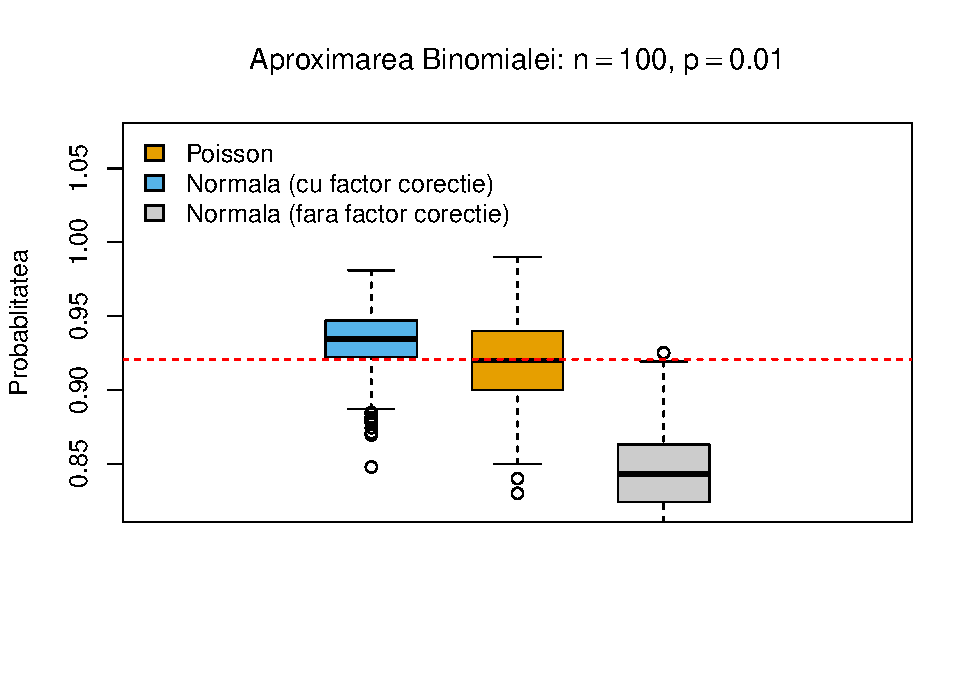
\includegraphics{Lab_4_files/figure-latex/unnamed-chunk-21-1} \end{center}


\end{document}
